\documentclass[border=10pt]{standalone}
\usepackage{tikz,amsmath}
\usetikzlibrary{arrows.meta}

% ========== 配色（Fill 填充 / Line 描边）==========
\definecolor{hidFill}{RGB}{199,203,243}
\definecolor{hidLine}{RGB}{52,58,143}
\definecolor{inFill}{RGB}{183,224,177}
\definecolor{inLine}{RGB}{32,102,32}
\definecolor{orFill}{RGB}{250,224,180}
\definecolor{orLine}{RGB}{190,110,20}
\definecolor{yeFill}{RGB}{252,240,180}
\definecolor{yeLine}{RGB}{180,150,20}
\definecolor{outFill}{RGB}{243,199,199}
\definecolor{outLine}{RGB}{143,52,52}

\begin{document}
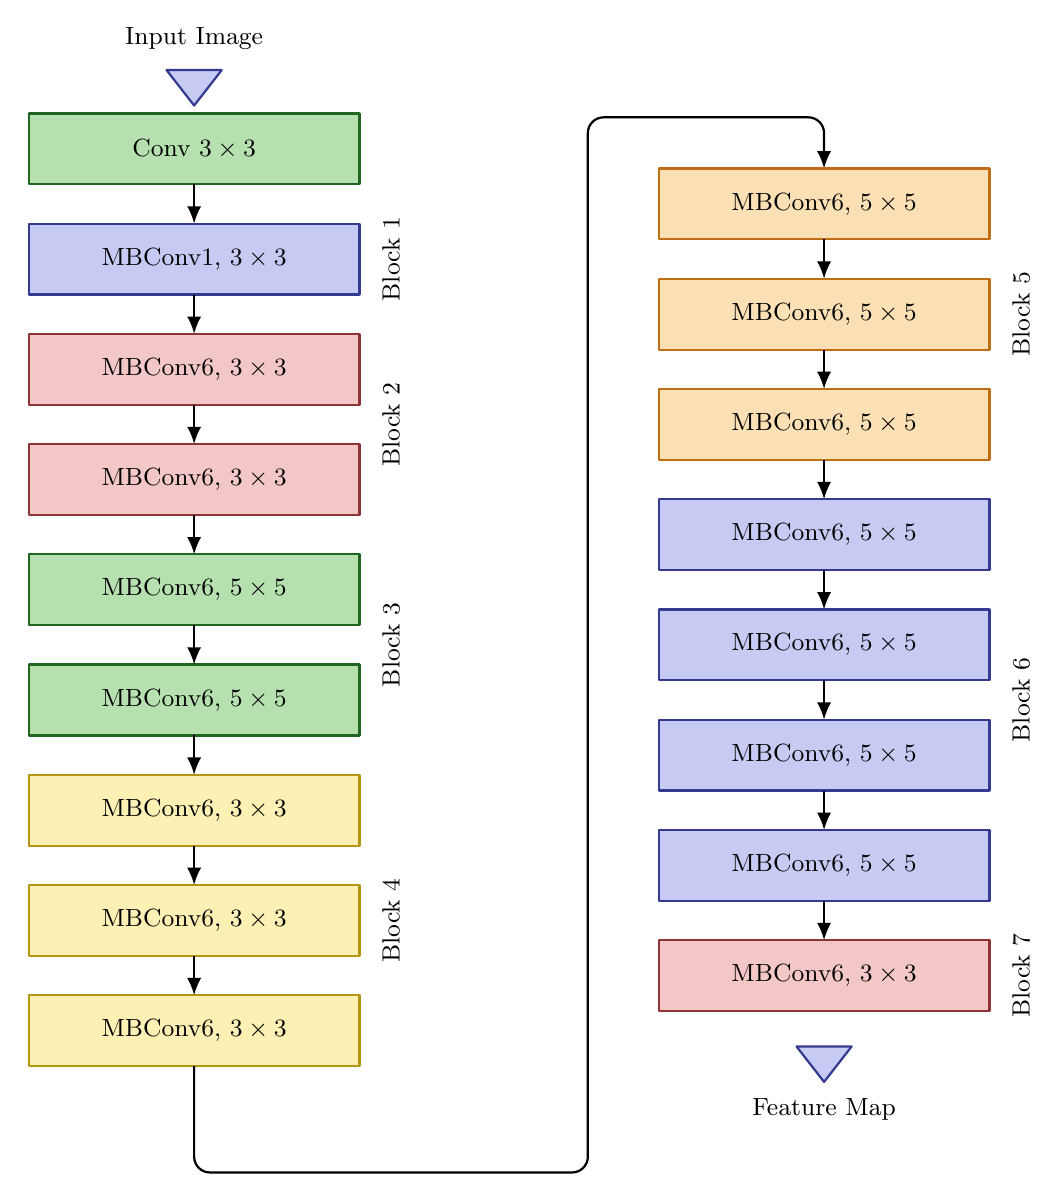
\begin{tikzpicture}[
    font=\small, line join=round,
    every node/.style={inner sep=0pt, outer sep=0pt, align=center},
    blk/.style={line width=.8pt, minimum width=4.2cm, minimum height=.9cm},
    arr/.style={-{Latex[length=2.2mm, width=1.8mm]}, line width=.8pt}
  ]

  % ========== 左列 ==========
  \node at (3,12.6) {Input Image};
  \fill[hidFill, draw=hidLine, line width=.8pt] (2.65,12.2) -- (3.35,12.2) -- (3,11.75) -- cycle;

  \foreach \y/\txt/\col in {
    11.2/{Conv $3\times3$}/in,
    9.8/{MBConv1, $3\times3$}/hid,
    8.4/{MBConv6, $3\times3$}/out,
    7.0/{MBConv6, $3\times3$}/out,
    5.6/{MBConv6, $5\times5$}/in,
    4.2/{MBConv6, $5\times5$}/in,
    2.8/{MBConv6, $3\times3$}/ye,
    1.4/{MBConv6, $3\times3$}/ye,
    0.0/{MBConv6, $3\times3$}/ye} {%
    \node[blk, fill=\col Fill, draw=\col Line] at (3,\y) {\txt};
  }
  \foreach \a/\b in {11.2/9.8, 9.8/8.4, 8.4/7.0, 7.0/5.6, 5.6/4.2, 4.2/2.8, 2.8/1.4, 1.4/0.0}
    \draw[arr] (3,\a-.45) -- (3,\b+.45);

  \node[rotate=90] at (5.5,9.8) {Block 1};
  \node[rotate=90] at (5.5,7.7) {Block 2};
  \node[rotate=90] at (5.5,4.9) {Block 3};
  \node[rotate=90] at (5.5,1.4) {Block 4};

  % ========== 回列折线：左列末 -> 右列首 ==========
  \draw[arr, rounded corners=2mm] (3,-0.45) -- (3,-1.8) -- (8,-1.8) -- (8,11.6) -- (11,11.6) -- (11,10.95);

  % ========== 右列 ==========
  \foreach \y/\txt/\col in {
    10.5/{MBConv6, $5\times5$}/or,
    9.1/{MBConv6, $5\times5$}/or,
    7.7/{MBConv6, $5\times5$}/or,
    6.3/{MBConv6, $5\times5$}/hid,
    4.9/{MBConv6, $5\times5$}/hid,
    3.5/{MBConv6, $5\times5$}/hid,
    2.1/{MBConv6, $5\times5$}/hid,
    0.7/{MBConv6, $3\times3$}/out} {%
    \node[blk, fill=\col Fill, draw=\col Line] at (11,\y) {\txt};
  }
  \foreach \a/\b in {10.5/9.1, 9.1/7.7, 7.7/6.3, 6.3/4.9, 4.9/3.5, 3.5/2.1, 2.1/0.7}
    \draw[arr] (11,\a-.45) -- (11,\b+.45);

  \node[rotate=90] at (13.5,9.1) {Block 5};
  \node[rotate=90] at (13.5,4.2) {Block 6};
  \node[rotate=90] at (13.5,0.7) {Block 7};

  % ========== 输出 ==========
  \fill[hidFill, draw=hidLine, line width=.8pt] (10.65,-0.2) -- (11.35,-0.2) -- (11,-0.65) -- cycle;
  \node at (11,-1.0) {Feature Map};

\end{tikzpicture}
\end{document}